\section{A Compelling Example}

Consider a sample nativity: \Sun, \Venus\xspace in \Cancer, \Moon, Ascendant in \Pisces, \Saturn\xspace in \Sagittarius,
the $<$preceding$>$ full moon, \Jupiter\xspace in \Capricorn, \Mars\xspace in \Scorpio, \Mercury\xspace in \Leo, the Lot of Fortune in \Leo, Daimon\xspace in \Scorpio
\footnote{\textit{Greek Horoscopes} dates the chart (L75) to approximately July 19, 75 AD (p.87). Also in Book III sections 6 and 14.}. 

\clearpage
\begin{wrapfigure}[15]{R}{7cm}
\centering
\vspace{-20pt}
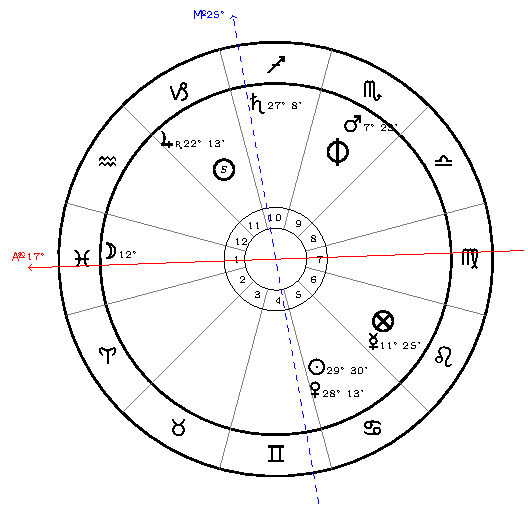
\includegraphics[width=0.68\textwidth]{charts/4_08_1}
\caption{Chart 42b [IV.08.1, GH L75]}
\label{fig:chart42b}
\end{wrapfigure} 

I am investigating the native’s 70th year. I count the chronocratorships relevant to health from \Leo\xspace $<$the Lot of Fortune$>$, first giving \Leo\xspace 19 years, then \Virgo\xspace 20, then \Libra\xspace 8, then \Scorpio\xspace 15. The total is 62 years. In these years he had many critical periods, falls from heights, and broken limbs \footnote{\Mars\xspace, ruler of accidents, injuries, is in \Scorpio}. 

I count off the remaining 8 years in \Sagittarius,\Saturn\xspace being there, not in its own sect. In these years he endured shipwrecks and bodily disorders. We learn the cause of the injury from the sign which the ruler of the Lot was found to be traversing: the Lot was in \Leo; the ruler of the Lot, the \Sun, was found in \Cancer. Now \Cancer\xspace indicates the breast and stomach, and so we say then that the cause of the injury was from \Cancer. 

\textbf{/159P/} Now he takes the allotment of years and converts it to 360 days. (After calculating the 5 1/4 days separately, add them to the years.) He gave \Sagittarius\xspace 1 year, \Capricorn\xspace 2 years 3 months, \Aquarius\xspace 2 years 6 months, \Pisces\xspace 1 year, then \Aries\xspace the remainder $<$2 years 3 months$>$ of the 9 years. \Mars, the current ruler of the chronocratorship for health, brings death, having received the chronocratorship from \Saturn\xspace located in \Sagittarius: \textbf{/168K/} he died diseased in the stomach and afflicted with coughing. The Place of Death was in \Pisces, with the \Moon\xspace there also and \Saturn\xspace in superior aspect, which caused the dysentery. In addition the ruler of the $<$preceding$>$ full moon, \Saturn, was turned away and caused the type of violent death. But the injury to the stomach and the cough resulted from the fact that the ruler of the Lot, the \Sun, was found in \Cancer, and \Cancer\xspace indicates breast and stomach.

Now I considered the chronocratorships for occupations, beginning with \Scorpio\xspace $<$=Daimon$>$, giving \Mars\xspace (which was in \Scorpio) 15 years, then \Sagittarius\xspace 12 years, with \Saturn\xspace in that sign. Until age 27 he was a vagrant, subject to ups and downs. His considerable property was squandered by his guardians, for
the $<$11th$>$ Place of Accomplishment was in \Gemini\xspace and no benefic was in aspect, but \Saturn\xspace was in
opposition. 

Next \Capricorn\xspace received the distribution of 27 years; \Jupiter\xspace was there, in $<$the XI Place of the$>$ Good Daimon, and it was in opposition to and beheld by the \Sun\xspace and \Venus. During this entire chronocratorship he had great success and was entrusted with public and royal affairs. He became a friend of governors and kings and became accordingly rich, but experienced setbacks and ups and downs in the course of time as a result of the malefics which received the allotment or were in aspect. His wealth was transitory because \Jupiter\xspace was found to be retrograde and in its depression $<$\Capricorn$>$. \Aquarius\xspace received
the distribution of the chronocratorship $<$at age 54$>$ after \Capricorn, with \Mars\xspace and \Mercury\xspace in aspect and
the benefics turned away. He ended his career and lost much through misplaced trust: he undertook pledges for relatives and slaves, through whose carelessness and poverty he fell into debt and was found abjectly poor, because the whole basis of the nativity aimed in this direction. 

\Aquarius\xspace took 2 years 6 months, then \Jupiter\xspace 1 year, then \Mars\xspace 1 year 3 months, then \Venus\xspace 8 months, then \Mercury\xspace 1 year 8 months. At that point his affairs went into a great decline. Next the \Moon\xspace received 2 years 1 month. During this period he seemed to recover some of his pledges and to get the help of friends. 

\textbf{/160P/} Next the \Sun\xspace received 1 year 7 months in \Leo, and \Mercury\xspace 1 year 8 months in \Virgo. Since malefics were in aspect with the Places $<$Accomplishment, Fortune$>$ and with \Mercury, he was ruined during this chronocratorship. The Lot of Fortune \textbf{/169K/} was found to be preceding an angle $<$the Descendant$>$, and the ruler of the triangle of the \Moon\xspace $<$\Cancer-\Pisces-\Scorpio$>$ was \Mars. 

Following \Mercury, \Venus\xspace received 8 months, then \Mars\xspace 1 years 3 months, then \Sagittarius\xspace 1 year. This was the end $<$69 years 4 months$>$.

\newpage